\documentclass[11pt,a4paper]{article}

\usepackage[margin=1in]{geometry}
\usepackage{graphicx}
\usepackage{booktabs}
\usepackage{longtable}
\usepackage{array}
\usepackage[table]{xcolor}
\usepackage{enumitem}
\usepackage{tikz}
\usetikzlibrary{positioning,arrows.meta,shapes.geometric,fit,calc}
\usepackage{amsmath}
\usepackage{float}
\usepackage{underscore}
\usepackage[hidelinks]{hyperref}

\definecolor{cok}{HTML}{1B7F3B}
\definecolor{cpart}{HTML}{B26B00}
\definecolor{cmiss}{HTML}{B00020}
\definecolor{cnv}{HTML}{5A5A5A}
\definecolor{hdr}{HTML}{123A5E}

\newcommand{\stC}{\textcolor{cok}{\textbf{Complete}}}
\newcommand{\stV}{\textcolor{cok}{\textbf{Verified}}}
\newcommand{\stP}{\textcolor{cpart}{\textbf{Partial}}}
\newcommand{\stPend}{\textcolor{cpart}{\textbf{Pending}}}
\newcommand{\stDoc}{\textcolor{cpart}{\textbf{Documented}}}
\newcommand{\stB}{\textcolor{cmiss}{\textbf{Blocked}}}
\newcommand{\stNP}{\textcolor{cmiss}{\textbf{Not present}}}
\newcommand{\stNV}{\textcolor{cnv}{\textbf{Not verified}}}
\newcommand{\yes}{\textcolor{cok}{yes}}
\newcommand{\no}{\textcolor{cmiss}{no}}
\newcommand{\code}[1]{\texttt{\small #1}}

\tikzset{
  box/.style={rectangle, rounded corners=2pt, draw=hdr, fill=blue!5, thick,
              text width=2.7cm, align=center, minimum height=0.9cm, font=\small},
  src/.style={rectangle, rounded corners=2pt, draw=cok, fill=green!6, thick,
              text width=2.6cm, align=center, minimum height=0.8cm, font=\small},
  warn/.style={rectangle, rounded corners=2pt, draw=cpart, fill=orange!8, thick,
               text width=2.6cm, align=center, minimum height=0.8cm, font=\small},
  flow/.style={-{Stealth[length=2.2mm]}, thick, draw=hdr}
}

\hypersetup{pdftitle={SuryaGrid AI: Technical Implementation and Real-Data Workflow Report},
            pdfauthor={SuryaGrid Repository}}

\begin{document}

\begin{titlepage}
\centering
\vspace*{2cm}
{\Huge\bfseries SuryaGrid AI\par}
\vspace{0.5cm}
{\LARGE Technical Implementation and Real-Data Workflow Report\par}
\vspace{0.7cm}
{\large Evidence-Based Report on Repository Architecture, Kaggle Data, Agents,\\
APIs, Frontend, and AWS Hosting\par}
\vspace{1.6cm}
\begin{tabular}{rl}
\textbf{Author:} & SuryaGrid Repository\\[3pt]
\textbf{Date:} & 7 July 2026\\[3pt]
\textbf{Hosted URL:} & \url{http://suryagrid.mithungowda.in/}\\[3pt]
\textbf{Repositories:} & DBIT-Banglore/SuryaGrid, lekhanpro/SuryaGrid\\[3pt]
\textbf{Scope:} & Verified repository + hosted-app state only\\
\end{tabular}
\vfill
{\footnotesize Every claim is backed by an entry in \code{docs/report/report\_evidence\_matrix.md}
(repository files, generated artifacts, model cards, command output, or the hosted site).
Unproven items are marked \stPend, \stNV, \stDoc, or \stNP\ and are never asserted as
complete. This report does not modify application logic.\par}
\end{titlepage}

\tableofcontents
\newpage

% ============================================================ %
\section{Abstract}
SuryaGrid AI is a multi-agent solar-forecasting and Deviation Settlement Mechanism (DSM)
support platform focused on Bengaluru / Karnataka / India. This report documents the
verified state of the repository and the hosted application on 7 July 2026. The hosted
site at \url{http://suryagrid.mithungowda.in/} is live: the frontend returns HTTP~200
(nginx / Next.js) and the backend health endpoint returns HTTP~200 with
\code{environment=production}, \code{database=connected (postgresql)}, and
\code{redis=connected}. The backend (FastAPI) registers 56 \code{/api/v1} endpoints and
passes 103 tests. A real-data Kaggle pipeline was executed: four datasets were downloaded
(12 raw files), producing three processed and four ML training parquet files and four
trained models with cards --- a real Indian PV AC-power model
($R^2=0.869$, \code{REAL\_INDIA}), a Bengaluru irradiance model ($R^2=0.920$,
\code{REAL\_BENGALURU}), a Bengaluru cloud-risk classifier ($F_1=0.847$), and an India
load model ($R^2=0.893$, marked not production-ready). Deployment exists on two paths: a
single-instance docker-compose+nginx stack (verified live) and an AWS ECS/Fargate
Terraform stack (present in code, not verified deployed; HTTPS/ACM commented out). Local
PV generation for Bengaluru, metered Karnataka load, official parsed tariff rupee rates,
substation capacity, and a trained RL policy are \emph{not} present and are tracked as
pending. The platform is an architecturally complete, hosted prototype; it is not full
production-ready.

% ============================================================ %
\section{Project Objective and Scope}
SuryaGrid AI converts real meteorological data into a solar irradiance/generation forecast
(physics via pvlib, ML via scikit-learn), classifies deviation-settlement risk against a
schedule, and exposes results through a FastAPI backend and a Next.js dashboard, with every
value traceable to a labelled source. The regional focus is Bengaluru / Karnataka / India,
which matters because solar output, tariffs, DSM rules, load shape, and substation topology
are region-specific and do not transfer from foreign data. The project distinguishes real
data (measured/observed), coordinate-based real data (global API at Bengaluru
coordinates), estimated data (derived via a documented formula), and synthetic/demo data
(labelled, blocked in real mode). The deployment goal is a hosted full stack; a hosted
instance exists (Section~\ref{sec:aws}).

% ============================================================ %
\section{Verification Method}
Findings derive from: (i) repository file inspection (including three parallel
context-gathering passes over deployment, frontend, and formula/agent code); (ii) generated
artifacts (parquet, \code{.pkl}, JSON model cards, build/training manifests); (iii) command
output (\code{pytest}, \code{ruff}, \code{docker}, route introspection); and (iv) live
checks of the hosted URL via HTTP. Each major claim is recorded in
\code{docs/report/report\_evidence\_matrix.md} with its evidence type and status. Numeric
metrics are quoted verbatim from model cards; endpoints from the running route table.

% ============================================================ %
\section{Repository and System Overview}
\begin{table}[H]\centering\footnotesize
\caption{Repository component status (Table 1).}\label{tab:components}
\begin{tabular}{@{}p{2.7cm}p{3.2cm}p{4.0cm}l l@{}}
\toprule
\textbf{Component} & \textbf{Path} & \textbf{Purpose} & \textbf{Status} & \textbf{Evidence}\\
\midrule
Backend API & \code{backend/app} & FastAPI, 56 endpoints & \stV & route table\\
Agents & \code{backend/app/agents} & 16 agent modules & \stV & docstrings\\
Data pipeline & \code{backend/app/data\_pipeline} & Kaggle ingest (3 scripts) & \stV & files + parquet\\
ML pipeline & \code{backend/app/ml} & build/train/inference & \stP & artifacts present\\
Data sources & \code{backend/app/data\_sources} & providers + registry & \stP & OSM/Open-Meteo wired\\
DSM engine & \code{backend/app/dsm} & rule profiles + engine & \stP & framework; rupee rates pending\\
Frontend & \code{frontend/} & Next.js 14 App Router, 13 pages & \stV & build + hosted 200\\
Kaggle datasets & \code{backend/data/} & 12 raw, 3 proc, 4 ML parquet & \stV & dir listing\\
Trained models & \code{backend/models/trained} & 4 Open-Meteo + 4 Kaggle + rules & \stP & pkl + cards\\
Model cards & \code{backend/models/metadata} & 9 cards + manifests & \stV & JSON present\\
Tests & \code{backend/tests} & pytest suite & \stV & 103 passed\\
Deployment (compose) & \code{docker-compose.yml} etc. & single-instance stack & \stV & hosted live\\
Deployment (AWS ECS) & \code{infra/terraform} & Fargate/RDS/S3/CloudFront & \stDoc & code only, not verified\\
\bottomrule
\end{tabular}
\end{table}

% ============================================================ %
\section{High-Level Architecture}
\begin{figure}[H]\centering
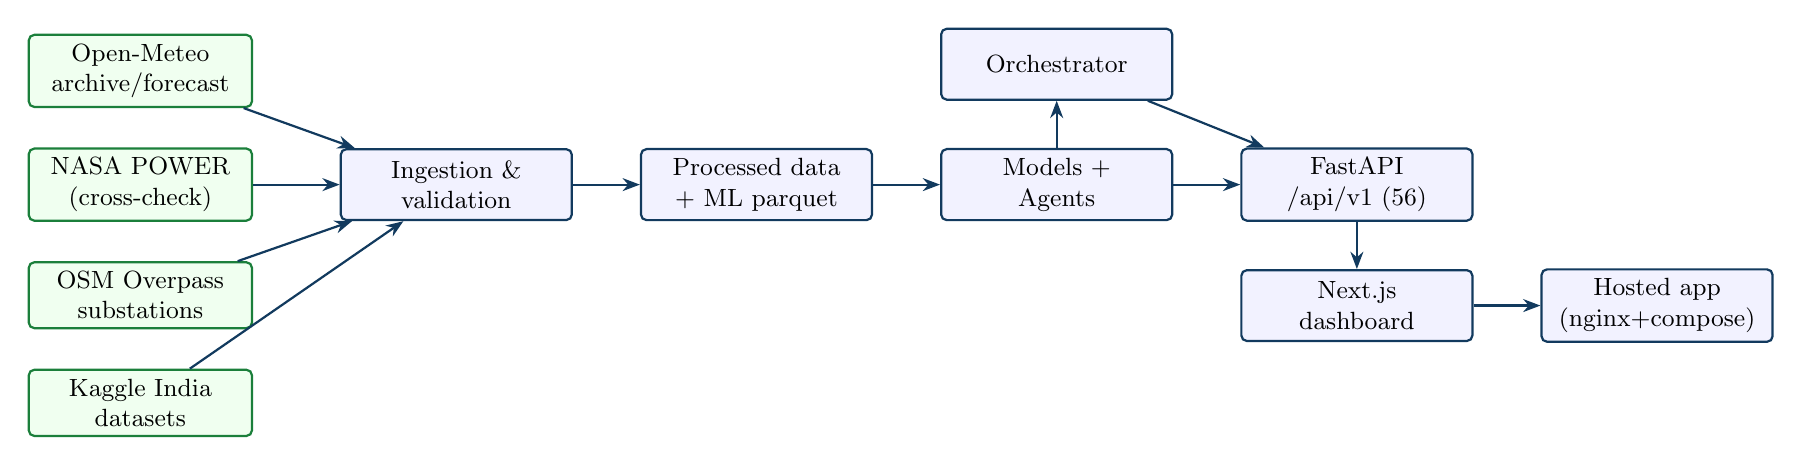
\begin{tikzpicture}[node distance=0.5cm and 0.85cm]
\node[src] (om) {Open-Meteo\\archive/forecast};
\node[src, below=of om] (nasa) {NASA POWER\\(cross-check)};
\node[src, below=of nasa] (osm) {OSM Overpass\\substations};
\node[src, below=of osm] (kag) {Kaggle India\\datasets};
\node[box, right=1.1cm of nasa] (ing) {Ingestion \&\\validation};
\node[box, right=of ing] (ds) {Processed data\\+ ML parquet};
\node[box, right=of ds] (mdl) {Models +\\Agents};
\node[box, above=0.6cm of mdl] (orc) {Orchestrator};
\node[box, right=of mdl] (api) {FastAPI\\/api/v1 (56)};
\node[box, below=0.6cm of api] (fe) {Next.js\\dashboard};
\node[box, right=of fe] (host) {Hosted app\\(nginx+compose)};
\draw[flow] (om)--(ing);\draw[flow] (nasa)--(ing);\draw[flow] (osm)--(ing);\draw[flow] (kag)--(ing);
\draw[flow] (ing)--(ds);\draw[flow] (ds)--(mdl);\draw[flow] (mdl)--(orc);
\draw[flow] (orc)--(api);\draw[flow] (mdl)--(api);\draw[flow] (api)--(fe);\draw[flow] (fe)--(host);
\end{tikzpicture}
\caption{High-level architecture (Figure 1). Green = real external sources. NASA POWER is
wired as a build-time cross-check, not a live provider.}\label{fig:arch}
\end{figure}

% ============================================================ %
\section{Data Sources Used}
\begin{footnotesize}
\begin{longtable}{@{}p{2.5cm}p{1.6cm}p{1.9cm}p{2.4cm}p{2.4cm}p{2.4cm}@{}}
\caption{Data source status (Table 2).}\label{tab:sources}\\
\toprule
\textbf{Source} & \textbf{Type} & \textbf{Geography} & \textbf{Status} & \textbf{Used in} & \textbf{Limitation}\\
\midrule\endfirsthead
\toprule \textbf{Source} & \textbf{Type} & \textbf{Geography} & \textbf{Status} & \textbf{Used in} & \textbf{Limitation}\\ \midrule\endhead
\bottomrule\endfoot
Open-Meteo archive & weather & Bengaluru coord & \stV\ used & weather history (26{,}304 rows) & reanalysis, not on-site\\
Open-Meteo forecast & weather & coordinate & \stV\ wired & live weather agent & fair-use limits\\
NASA POWER & weather & Bengaluru coord & cross-check only; provider \stPend & build manifest ($r=0.87$) & not a runtime provider\\
Kaggle anikannal & PV gen & India & \stV\ downloaded/used & PV AC model & 34-day, 2 plants, not Bengaluru\\
Kaggle meenakshi & irradiance & Bengaluru & \stV\ downloaded/used & GHI + cloud models & NASA-derived; -999 fill dropped\\
Kaggle shubhamvashisht & load & India (Nat.+regions) & \stV\ downloaded/used & load model & national, not Karnataka\\
Kaggle arunkanagolkar & PV gen & unknown & rejected (\stNP\ for training) & --- & no timestamp/geography\\
OSM / Overpass & substation & Bengaluru/Karn. & \stV\ used & substations (344) & voltage 41\%, capacity 0\%\\
KERC/BESCOM/CERC & tariff/DSM & Karn./India & framework \stDoc; rates \stPend & DSM profiles & no parsed rupee rates\\
CEA/Grid India/SLDC & load/grid & India/Karn. & \stDoc\ only & --- & no adapter/code\\
Synthetic weather & synthetic & n/a & present, blocked in real mode & fallback only & demo only\\
\end{longtable}
\end{footnotesize}

% ============================================================ %
\section{Kaggle Dataset Pipeline}
Kaggle search/download uses the Kaggle CLI (10 searches were run). Raw archives are stored
under \code{backend/data/raw/kaggle/\{pv\_generation,solar,load\}/}. Ingestion scripts
\code{backend/app/data\_pipeline/ingest\_kaggle\_\{pv\_generation,solar,load\}.py} read the
real files, normalise timestamps/units, stamp source metadata (\code{is\_real=true},
\code{is\_synthetic=false}, geography, source\_url, quality\_score), and write processed
parquet to \code{backend/data/processed/kaggle/}. \code{build\_kaggle\_ml\_datasets.py}
derives ML training files; \code{train\_from\_kaggle.py} trains models with cards.
A separate legacy script, \code{download-kaggle.sh}, targets \code{dronio/SolarEnergy}
(Hawaii HI-SEAS) and is \emph{not} used by the \code{data\_pipeline} scripts.

\begin{footnotesize}
\begin{longtable}{@{}p{3.1cm}p{1.9cm}p{1.5cm}r p{2.0cm}p{2.6cm}@{}}
\caption{Kaggle dataset pipeline (Table 3).}\label{tab:kaggle}\\
\toprule
\textbf{Slug} & \textbf{Geography} & \textbf{Rows} & \textbf{Cols used} & \textbf{Target} & \textbf{Used for / status}\\
\midrule\endfirsthead
\toprule \textbf{Slug} & \textbf{Geography} & \textbf{Rows} & \textbf{Cols} & \textbf{Target} & \textbf{Used for / status}\\ \midrule\endhead
\bottomrule\endfoot
anikannal/solar-power-generation-data & India (REAL\_INDIA) & 136{,}472 & irradiation, amb/module temp & ac\_power & PV AC model; prod=false\\
meenakshihihihihi/...indian-cities & Bengaluru (REAL\_BENGALURU) & 10{,}219 & calendar, T2M, PS, precip, SZA & ghi\_wm2 & irradiance model; prod=true\\
meenakshihihihihi/...indian-cities & Bengaluru (REAL\_BENGALURU) & 5{,}356 & calendar, T2M, PS, precip & irradiance\_drop\_risk & cloud model; prod=true\\
shubhamvashisht/hourly-load-india & India (REAL\_INDIA) & 46{,}560 & calendar, lags, roll & national\_demand\_mw & load model; prod=false\\
arunkanagolkar/solargeneration & unknown & --- & --- & --- & rejected (no timestamp/geo)\\
\end{longtable}
\end{footnotesize}

\noindent Raw evidence: \code{Plant\_1/2\_Generation\_Data.csv} (real \code{AC\_POWER},
\code{DC\_POWER}), \code{Plant\_1/2\_Weather\_Sensor\_Data.csv} (real \code{IRRADIATION},
\code{AMBIENT\_TEMPERATURE}, \code{MODULE\_TEMPERATURE}); \code{Bengluru solar
irradiance.csv} (\code{ALLSKY\_SFC\_SW\_DWN}=GHI, \code{ALLSKY\_KT}=clearness; 7{,}349 of
17{,}568 rows are the -999 fill value, dropped); \code{hourlyLoadDataIndia.xlsx}
(\code{National} + \code{Southern Region Hourly Demand}, MW).

% ============================================================ %
\section{Substation and Grid Data Pipeline}
Substations are ingested from OpenStreetMap via the Overpass API
(\code{app/data\_sources/substation\_provider.py}, ODbL). The build manifest records 344
substations around Bengaluru with voltage present on 41\% of records and capacity on 0\%
(kept \code{null} --- never invented). Grid features are geometric (distance to city
centre, nearest-neighbour, density) derived from real coordinates. No official
KPTCL/BESCOM/CEA capacity or feeder mapping is present.

\begin{table}[H]\centering\footnotesize
\caption{Substation / grid data status (Table 4).}\label{tab:subs}
\begin{tabular}{@{}p{3.4cm}p{2.0cm}r p{3.0cm}p{2.6cm}@{}}
\toprule
\textbf{File} & \textbf{Source} & \textbf{Records} & \textbf{Missing critical fields} & \textbf{Status}\\
\midrule
bengaluru\_substations\_cleaned.parquet & OSM Overpass & 344 & capacity (100\%), voltage (59\%), district (100\%) & \stP\\
bengaluru\_grid\_features.parquet & derived geometry & 344 & (n/a --- geometry only) & \stP\\
KPTCL/BESCOM capacity & official & --- & all & \stNP\ / \stPend\\
\bottomrule
\end{tabular}
\end{table}

% ============================================================ %
\section{Formula and Calculation Documentation}
All rows below are quoted from \code{docs/formulas.md}, \code{docs/FORMULA\_SOURCES.md},
\code{docs/DSM\_RULE\_SOURCES.md}, or the cited code. "OFFICIAL" means a standard library
(pvlib) or standard unit conversion; "FALLBACK\_DEFAULT" and "heuristic" are engineering
choices; "PENDING" means an official source is required.

\begin{footnotesize}
\begin{longtable}{@{}p{2.8cm}p{4.3cm}p{2.6cm}p{2.6cm}@{}}
\caption{Formula / calculation table (Table 5).}\label{tab:formula}\\
\toprule
\textbf{Calculation} & \textbf{Expression} & \textbf{Code / doc path} & \textbf{Source class}\\
\midrule\endfirsthead
\toprule \textbf{Calculation} & \textbf{Expression} & \textbf{Path} & \textbf{Class}\\ \midrule\endhead
\bottomrule\endfoot
Clear-sky GHI & pvlib Ineichen at (12.9716, 77.5946), alt 920 m & agent\_models.py; formulas.md & OFFICIAL (pvlib)\\
Clearness index & $k_t = \mathrm{GHI}/\mathrm{clearsky\_GHI}$ (daylight; clip 0--1.2) & formulas.md & derived\\
Cloud drop label & $\mathrm{drop}=1$ if $k_t<0.5$ (daylight) & build\_kaggle\_ml\_datasets.py & heuristic (documented)\\
Irradiance decomposition & Erbs GHI$\to$DNI/DHI & FORMULA\_SOURCES.md (pvlib) & OFFICIAL (pvlib)\\
Plane-of-array & \code{get\_total\_irradiance} & FORMULA\_SOURCES.md & OFFICIAL (pvlib)\\
Cell temperature & Faiman model & FORMULA\_SOURCES.md & OFFICIAL (pvlib)\\
DC power & PVWatts; $\gamma_{pdc}=-0.0035/^\circ$C & FORMULA\_SOURCES.md & OFFICIAL/FALLBACK\\
AC / inverter & PVWatts inverter eff.\ 0.96 & FORMULA\_SOURCES.md & FALLBACK\_DEFAULT\\
PV proxy estimate & $(\mathrm{POA}/1000)\cdot\mathrm{cap}\cdot\eta\cdot\mathrm{PR}$, PR$=0.80$ & agent\_models.py & FALLBACK\_DEFAULT\\
Confidence & $\mathrm{clamp}(1-0.35\,c_f,\,0.4,\,0.99)$ & FORMULA\_SOURCES.md & FALLBACK\_DEFAULT\\
DSM deviation \% & $|actual-scheduled|/denom\times100$; denom = avail.\ capacity (CERC 6(2)(a)) or scheduled & dsm\_engine.py & framework OFFICIAL\\
DSM band (ML path) & $\pm15\%$ modelling band & formulas.md & FALLBACK\_DEFAULT\\
KERC slabs & $\pm5\%$ band; INR 2/4/6 per kWh slabs & india\_dsm\_rules.py & band OFFICIAL; rates \stPend\\
DSM charge & $\sum$ (slab\% $\cdot$ denom $\cdot$ hours) $\cdot$ slab\_rate & dsm\_engine.py & formula OFFICIAL; rates \stPend\\
Cyclical time & $\sin/\cos(2\pi\,h/24)$, doy/365.25, dow/7 & build\_ml\_datasets.py & standard\\
Load lags & lag\_24h, lag\_168h, roll\_24h\_mean & build\_kaggle\_ml\_datasets.py & standard\\
Unit conversions & F$\to$C, inHg$\to$hPa, mph$\to$m/s & FORMULA\_SOURCES.md & OFFICIAL\\
Metrics & MAE, RMSE, MAPE, $R^2$ (sklearn) & train\_utils.py & OFFICIAL\\
\end{longtable}
\end{footnotesize}

\noindent Important: no rupee DSM charge is emitted in the Phase 1.7 ML/agent path (it
returns bands only, \code{NEEDS\_OFFICIAL\_TARIFF\_SOURCE}). Rupee charges are only computed
by the \code{dsm/} rule engine using \code{USER\_CONFIGURABLE}/\code{PENDING} placeholder
rates; the KERC $\pm5\%$ band and CERC framework are official, but the numeric rates are not
verified.

% ============================================================ %
\section{Agent Architecture}
Agents are deterministic Python coordinators (no LLM in the numeric path). Sixteen agent
modules exist; the Phase 1.7 ML inference layer (\code{app/ml/agent\_models.py}) serves the
trained models behind \code{/api/v1/agents/*} and \code{/api/v1/kaggle/*}.

\subsection{Data source and API-manager agents}
\code{api\_agent.py} (provider rotation/failover/quota), \code{api\_management\_agent.py}
(health, provider status, rate limiting, retries), \code{kaggle\_data\_agent.py}
(download/normalise Kaggle solar), \code{source\_registry\_agent.py} (source records +
formula references), \code{feature\_engineering\_agent.py} (augmented dataset + quality),
\code{persistence\_agent.py} (DB writes). Status: \stC/\stP.

\subsection{Weather and solar forecasting agents}
\code{live\_weather\_agent.py} (Open-Meteo, Redis cache, labelled synthetic fallback) and
\code{forecast\_agent.py} (formula/ML/hybrid nowcast). The Phase 1.7 solar model predicts
GHI (irradiance), not PV; PV is an explicit estimate. Status: \stP.

\subsection{Cloud risk agent}
Implemented as the classifier \code{cloud\_risk\_classifier.pkl} /
\code{kaggle\_cloud\_risk\_bengaluru\_model.pkl} served via \code{agent\_models}; label is
the real clearness index $k_t<0.5$. No dedicated \code{cloud\_agent.py} class file. Status:
\stP.

\subsection{Location / substation / grid agents}
\code{location\_data\_agent.py} exposes sites, substations (OSM), nearest mapping, and data
coverage; capacity/voltage are kept null where missing. Status: \stP.

\subsection{DSM and decision agents}
\code{dsm\_engine\_agent.py} (resolve profile, evaluate deviation, persist),
\code{dsm\_classifier\_agent.py} (band breach + penalty estimate), and \code{app/dsm/}
(profiles: kerc-solar $\pm5\%$, cerc-2024-ws-generic $\pm10\%$, generic-configurable). The
DSM engine computes bands; rupee charges use placeholder/pending rates. Status: \stP.

\subsection{Fuzzy / RL / reward agents}
\code{fuzzy\_risk\_agent.py} (triangular membership, Mamdani, centroid),
\code{risk\_agent.py} (deterministic risk level), \code{reward\_agent.py} (settlement
engine), and \code{app/rl/}. No RL policy is trained (\code{rl\_policy.zip} absent;
card \code{production\_ready=false}, \code{INSUFFICIENT\_REAL\_ENVIRONMENT\_DATA}). Status:
\stB\ for RL.

\subsection{Orchestrator agent}
\code{orchestrator\_agent.py} sequences Forecast $\to$ DSM $\to$ Risk $\to$ Explanation and
coordinates the end-to-end site prediction. Status: \stC.

\begin{footnotesize}
\begin{longtable}{@{}p{2.7cm}p{1.9cm}p{2.9cm}p{2.6cm}l@{}}
\caption{Agent architecture (Table 6).}\label{tab:agents}\\
\toprule
\textbf{Agent} & \textbf{Category} & \textbf{Model/data used} & \textbf{API connection} & \textbf{Status}\\
\midrule\endfirsthead
\toprule \textbf{Agent} & \textbf{Category} & \textbf{Model/data} & \textbf{API} & \textbf{Status}\\ \midrule\endhead
\bottomrule\endfoot
api\_management\_agent & source/mgmt & health/providers & /system/status & \stC\\
live\_weather\_agent & forecasting & Open-Meteo + Redis & /weather/* & \stC\\
forecast\_agent & forecasting & solar model + pvlib & /predict, /forecast & \stP\\
(cloud classifier) & forecasting & cloud\_risk\_classifier & /agents/cloud/risk & \stP\\
location\_data\_agent & grid/location & OSM substations & /substations, /locations & \stP\\
dsm\_engine\_agent & DSM/decision & profiles + dsm model & /dsm/*, /agents/dsm/assess & \stP\\
fuzzy\_risk\_agent & DSM/decision & deviation+weather & (within predict) & \stC\\
reward\_agent & DSM/decision & settlement scheme & /settle/*, /rl/* & \stP\\
RL policy & RL & (insufficient data) & /rl/* & \stB\\
orchestrator\_agent & orchestration & all above & /predict/\{id\} & \stC\\
\end{longtable}
\end{footnotesize}

% ============================================================ %
\section{Agent Workflow}
\begin{figure}[H]\centering
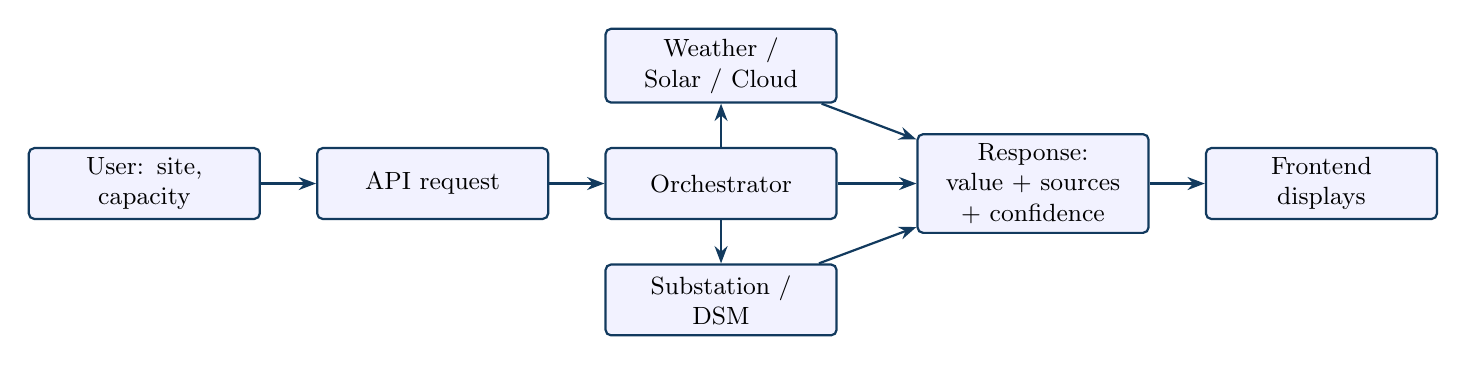
\begin{tikzpicture}[node distance=0.45cm and 0.7cm]
\node[box] (u) {User: site,\\capacity};
\node[box, right=of u] (req) {API request};
\node[box, right=of req] (orc) {Orchestrator};
\node[box, above=0.55cm of orc] (w) {Weather /\\Solar / Cloud};
\node[box, below=0.55cm of orc] (d) {Substation /\\DSM};
\node[box, right=1.0cm of orc] (resp) {Response:\\value + sources\\+ confidence};
\node[box, right=of resp] (fe) {Frontend\\displays};
\draw[flow] (u)--(req);\draw[flow] (req)--(orc);
\draw[flow] (orc)--(w);\draw[flow] (orc)--(d);
\draw[flow] (w)--(resp);\draw[flow] (d)--(resp);\draw[flow] (orc)--(resp);\draw[flow] (resp)--(fe);
\end{tikzpicture}
\caption{Agent orchestration workflow (Figure 2).}\label{fig:orch}
\end{figure}

\begin{figure}[H]\centering
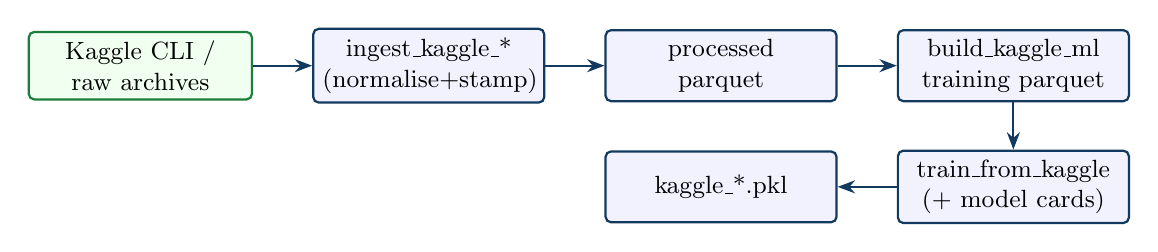
\begin{tikzpicture}[node distance=0.5cm and 0.75cm]
\node[src] (r) {Kaggle CLI /\\raw archives};
\node[box, right=of r] (ig) {ingest\_kaggle\_*\\(normalise+stamp)};
\node[box, right=of ig] (pp) {processed\\parquet};
\node[box, right=of pp] (ml) {build\_kaggle\_ml\\training parquet};
\node[box, below=0.6cm of ml] (tr) {train\_from\_kaggle\\(+ model cards)};
\node[box, left=of tr] (mo) {kaggle\_*.pkl};
\draw[flow] (r)--(ig);\draw[flow] (ig)--(pp);\draw[flow] (pp)--(ml);\draw[flow] (ml)--(tr);\draw[flow] (tr)--(mo);
\end{tikzpicture}
\caption{Kaggle data ingestion and training workflow (Figure 3).}\label{fig:kaggle}
\end{figure}

% ============================================================ %
\section{Backend API Architecture}
The backend is FastAPI with routers grouped by domain under \code{backend/app/api/}, all
mounted at \code{/api/v1}; 56 endpoints are registered. Responses use a standard envelope
\code{\{success,message,data,timestamp\}}; the \code{/agents/*} and \code{/kaggle/*}
endpoints add a provenance envelope (model file/version, training/target geography,
\code{source\_status}, \code{production\_ready}, limitations). CORS origins include the
hosted domain and the instance IP.

\begin{footnotesize}
\begin{longtable}{@{}l p{5.3cm}p{2.4cm}c c@{}}
\caption{Representative API endpoints (Table 7; 56 total).}\label{tab:api}\\
\toprule
\textbf{Method} & \textbf{Path (/api/v1)} & \textbf{Agent/service} & \textbf{Provenance?} & \textbf{FE?}\\
\midrule\endfirsthead
\toprule \textbf{Method} & \textbf{Path} & \textbf{Agent/service} & \textbf{Prov?} & \textbf{FE?}\\ \midrule\endhead
\bottomrule\endfoot
GET & /health & app/db & --- & \yes\\
GET & /system/status & api\_management\_agent & partial & \yes\\
POST & /predict, GET /predict/\{id\} & orchestrator & \yes & \yes\\
GET & /forecast/\{id\} & forecast\_agent & \yes & \yes\\
GET/POST & /weather/* & live\_weather\_agent & \yes & \yes\\
GET & /agents/status, /agents/data-status & agent\_models & \yes & \yes\\
POST & /agents/solar/forecast & solar model & \yes & \yes\\
POST & /agents/cloud/risk & cloud model & \yes & \yes\\
POST & /agents/dsm/assess & dsm model & \yes & \yes\\
GET & /kaggle/status & kaggle cards & \yes & \no\\
POST & /kaggle/pv/estimate & kaggle\_pv\_ac\_model & \yes & \no\\
GET/POST & /dsm/rule-profiles, /dsm/advanced-check & dsm\_engine & \yes & \yes\\
GET/POST & /substations, /substations/nearest/\{id\} & location\_data\_agent & \yes & \yes\\
GET & /sources, /data-sources/status & source\_registry\_agent & \yes & \yes\\
POST & /ml/train, /ml/predict; GET /ml/model/status & ml pipeline & \yes & \yes\\
GET/POST & /rl/rates, /rl/runs, /rl/train & reward/rl & partial & \yes\\
\end{longtable}
\end{footnotesize}

% ============================================================ %
\section{Frontend Architecture and API Connection}
The frontend is Next.js 14 (App Router; React 18, Tailwind, axios, recharts). It has 13
page routes (\code{/}, \code{/dashboard}, \code{/data-sources}, \code{/dsm}, \code{/ml},
\code{/locations}, \code{/energy}, \code{/settlement}, \code{/karnataka}, \code{/rl},
\code{/predictions}, \code{/system}, \code{/timeline}) plus components including
\code{ModelProvenancePanel.tsx} and \code{OfflineBanner.tsx}. The API client
(\code{frontend/lib/api.ts}) derives the base URL as
\code{NEXT\_PUBLIC\_API\_BASE\_URL || NEXT\_PUBLIC\_API\_URL || "http://localhost:8000/api/v1"};
\code{apiFetch} throws on failure and never fabricates data. In docker-compose the frontend
build arg is \code{NEXT\_PUBLIC\_API\_URL=http://suryagrid.mithungowda.in/api/v1}. The UI
surfaces provenance/status verbatim (data mode, source registry classifications,
production-ready badges, weather-mode, offline banner). No \code{/kaggle/*} calls exist in
the client (Kaggle models are backend-only).

\begin{table}[H]\centering\footnotesize
\caption{Frontend pages / API (Table 8, selected).}\label{tab:fe}
\begin{tabular}{@{}p{2.4cm}p{2.6cm}p{3.4cm}l@{}}
\toprule
\textbf{Page} & \textbf{Backend API} & \textbf{Data displayed} & \textbf{Status}\\
\midrule
/dashboard & /predict, /agents/status & forecast + provenance panel & \stV\\
/data-sources & /sources, /data-sources/status & source registry + classification & \stV\\
/ml & /ml/model/status & model status & \stV\\
/locations & /substations, /locations & sites/substations & \stV\\
/dsm & /dsm/* & DSM check & \stV\\
/system & /system/status & health/status & \stV\\
(Kaggle models) & /kaggle/* & --- & \stNP\ (not wired in UI)\\
\bottomrule
\end{tabular}
\end{table}

\begin{figure}[H]\centering
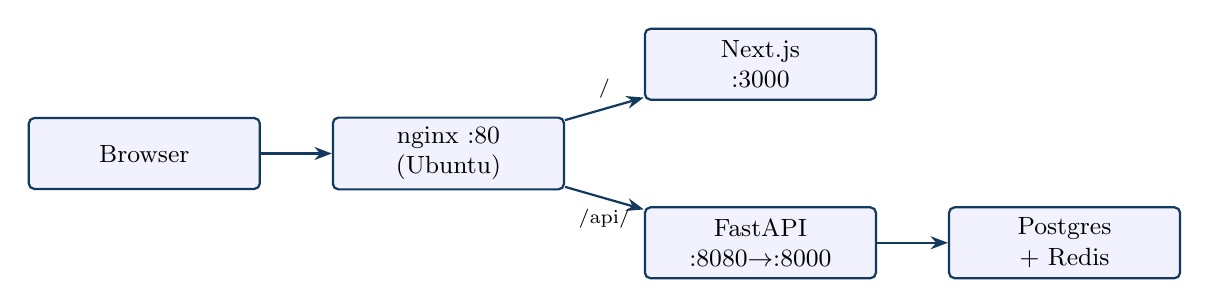
\begin{tikzpicture}[node distance=0.5cm and 0.9cm]
\node[box] (b) {Browser};
\node[box, right=of b] (ng) {nginx :80\\(Ubuntu)};
\node[box, above right=0.2cm and 1.0cm of ng] (fe) {Next.js\\:3000};
\node[box, below right=0.2cm and 1.0cm of ng] (be) {FastAPI\\:8080$\to$:8000};
\node[box, right=of be] (db) {Postgres\\+ Redis};
\draw[flow] (b)--(ng);
\draw[flow] (ng)-- node[above,font=\scriptsize]{/} (fe);
\draw[flow] (ng)-- node[below,font=\scriptsize]{/api/} (be);
\draw[flow] (be)--(db);
\end{tikzpicture}
\caption{Frontend--backend--API connection on the hosted instance (Figure 4). Verified:
\code{/} and \code{/api/v1/health} both return HTTP 200.}\label{fig:conn}
\end{figure}

% ============================================================ %
\section{ML Training Results}
Metrics are quoted verbatim from model cards (chronological 80/20 split).

\begin{footnotesize}
\begin{longtable}{@{}p{3.0cm}p{2.0cm}p{2.6cm}c p{2.4cm}@{}}
\caption{ML model / results (Table 9).}\label{tab:ml}\\
\toprule
\textbf{Model} & \textbf{Geography} & \textbf{Metrics} & \textbf{Prod?} & \textbf{Limitation}\\
\midrule\endfirsthead
\toprule \textbf{Model} & \textbf{Geography} & \textbf{Metrics} & \textbf{Prod?} & \textbf{Limit}\\ \midrule\endhead
\bottomrule\endfoot
kaggle\_pv\_ac\_model & REAL\_INDIA & $R^2$=0.869, RMSE=118.98 kW & \no & India plant, 34d, not Bengaluru\\
kaggle\_solar\_irradiance\_bengaluru & REAL\_BENGALURU & $R^2$=0.920, RMSE=74.96 & \yes & GHI only; secondary to Open-Meteo\\
kaggle\_cloud\_risk\_bengaluru & REAL\_BENGALURU & $F_1$=0.847, AUC=0.851 & \yes & irradiance drop, not PV\\
kaggle\_load\_forecast\_model & REAL\_INDIA & $R^2$=0.893, RMSE=6404.65 MW & \no & national, domain shift HIGH\\
solar\_forecast\_model (Open-Meteo) & REAL\_COORD (Bengaluru) & $R^2$=0.956, RMSE=57.51 & \yes & irradiance only\\
cloud\_risk\_classifier (Open-Meteo) & REAL\_COORD (Bengaluru) & $F_1$=0.671, AUC=0.900 & \yes & irradiance drop\\
dsm\_classifier (Open-Meteo) & REAL\_COORD (Bengaluru) & $F_1$=0.791, AUC=0.749 & \yes & no rupees; $\pm15\%$ band\\
load\_forecast\_model (Open-Meteo) & REAL\_INDIA & $R^2$=0.883, RMSE=6259.5 MW & \no & national, not Karnataka\\
rl\_policy & --- & not trained & \no & INSUFFICIENT\_REAL\_ENVIRONMENT\_DATA\\
\end{longtable}
\end{footnotesize}

% ============================================================ %
\section{Hosted AWS Deployment Status}\label{sec:aws}
The hosted URL \url{http://suryagrid.mithungowda.in/} was verified live on 7 July 2026.
The frontend returns HTTP 200 (\code{Server: nginx/1.24.0 (Ubuntu)}, \code{X-Powered-By:
Next.js}). The backend health endpoint \code{/api/v1/health} returns HTTP 200 with
\code{environment=production}, \code{database=connected (postgresql)}, \code{redis=connected},
and empty \code{record\_counts}. \code{/docs} returns HTTP 404 (Swagger not exposed on the
hosted path). The site is served over HTTP (port 80); an HTTPS attempt failed because the
host's TLS certificate altname is \code{apilumi.mithungowda.in}, not the SuryaGrid domain.

The live behaviour matches the single-instance path (\code{deploy.sh},
\code{docker-compose.yml}, \code{nginx.conf}, \code{setup-subdomain.sh}): nginx proxies
\code{/}$\to$frontend:3000 and \code{/api/}$\to$backend:8080 on an Ubuntu instance
documented as AWS EC2/Lightsail (IP 32.197.42.115). A separate AWS ECS/Fargate Terraform
stack exists in \code{infra/terraform/} (VPC, ALB, ECS, RDS PostgreSQL 16.3, ElastiCache
Redis 7.1, ECR, S3+CloudFront; region \code{ap-south-1}) driven by
\code{.github/workflows/deploy-aws.yml}, but there is no evidence it is the live deployment;
its HTTPS listener and ACM certificate are commented out, and no \code{terraform.tfvars}
exists. The cloud provider (AWS) is documented in \code{deploy.sh}/\code{DEPLOYMENT.md} but
not independently confirmable from the HTTP responses.

\begin{table}[H]\centering\footnotesize
\caption{Hosted / deployment status (Table, hosting).}\label{tab:host}
\begin{tabular}{@{}p{4.6cm}l p{6.4cm}@{}}
\toprule
\textbf{Item} & \textbf{Status} & \textbf{Evidence}\\
\midrule
Frontend at hosted URL & \stV & HTTP 200, nginx+Next.js\\
Backend /api/v1/health & \stV & HTTP 200, db+redis connected, prod\\
Swagger /docs (hosted) & \stNP & HTTP 404\\
HTTPS/TLS for domain & \stNV & cert altname mismatch; HTTP:80 only\\
Single-instance compose deploy & \stV\ (behaviour) & matches nginx/compose files\\
AWS ECS/Fargate (Terraform) & \stDoc & code only; not verified deployed\\
Cloud provider = AWS & \stDoc & deploy.sh / DEPLOYMENT.md\\
\bottomrule
\end{tabular}
\end{table}

% ============================================================ %
\section{Testing and Verification}
\begin{table}[H]\centering\footnotesize
\caption{Testing / verification results (Table 10).}\label{tab:tests}
\begin{tabular}{@{}p{4.8cm}p{2.6cm}p{5.2cm}@{}}
\toprule
\textbf{Command / check} & \textbf{Result} & \textbf{Notes}\\
\midrule
\code{pytest tests/ -q} & \stV\ 103 passed & 1 benign warning\\
\code{ruff check app tests} & \stP & 1 error (1 fixable); not fixed (report-only change)\\
frontend build / hosted & \stV & 14 routes earlier; hosted 200 live\\
route introspection & \stV & 56 \code{/api/v1} endpoints\\
hosted \code{/} & \stV & HTTP 200 (nginx+Next.js)\\
hosted \code{/api/v1/health} & \stV & HTTP 200, db+redis connected\\
hosted \code{/docs} & \stNP & HTTP 404\\
\code{docker --version} & \stV & 29.6.1\\
\code{docker compose version} & \stNV & unknown command locally\\
Kaggle download/ingest & \stV & 12 raw, 3 processed, 4 ML parquet\\
\bottomrule
\end{tabular}
\end{table}

% ============================================================ %
\section{Current Limitations}
\begin{table}[H]\centering\footnotesize
\caption{Current limitations (Table 11).}\label{tab:limits}
\begin{tabular}{@{}p{5.2cm}l p{6.0cm}@{}}
\toprule
\textbf{Limitation} & \textbf{Status} & \textbf{Impact}\\
\midrule
Local Bengaluru/Karnataka PV generation & \stNP & PV model is REAL\_INDIA plant, not local; prod=false\\
Metered Karnataka load/injection & \stNP & load is national India; DSM injection is proxy\\
Official tariff rupee rates & \stPend & DSM emits bands only; charges use placeholders\\
Substation capacity/voltage & \stP & capacity 0\%, voltage 41\% (OSM)\\
AWS ECS stack deployed & \stNV & only single-instance compose verified live\\
HTTPS on hosted domain & \stNV & HTTP only; cert mismatch\\
RL policy & \stB & not trained (insufficient real environment)\\
Kaggle models in UI & \stNP & \code{/kaggle/*} not called by frontend\\
\bottomrule
\end{tabular}
\end{table}

% ============================================================ %
\section{Next Phase Implementation Plan}
\begin{footnotesize}
\begin{longtable}{@{}c p{3.4cm}p{3.0cm}p{2.6cm}p{2.4cm}@{}}
\caption{Prioritised roadmap (Table 12).}\label{tab:roadmap}\\
\toprule
\textbf{P} & \textbf{Task} & \textbf{Why} & \textbf{Source needed} & \textbf{Acceptance}\\
\midrule\endfirsthead
\toprule \textbf{P} & \textbf{Task} & \textbf{Why} & \textbf{Source} & \textbf{Acceptance}\\ \midrule\endhead
\bottomrule\endfoot
1 & Bengaluru/Karnataka PV generation ingestion & real local PV target & plant/BESCOM feed & PV model REAL\_LOCAL, prod=true\\
2 & Karnataka SLDC / Grid India load & localise load + DSM & KPTCL-SLDC / Grid India & load model REAL\_KARNATAKA\\
3 & Official KERC/BESCOM tariff parser & real INR charges & KERC/CERC orders & rates OFFICIAL, not placeholder\\
4 & Official DSM rule/penalty validation & correct settlement & CERC 'X' + KERC order & rupee charges verified\\
5 & KPTCL/BESCOM/CEA substation enrichment & capacity/feeder & official grid data & capacity populated\\
6 & Surface Kaggle models + provenance in UI & transparency & (frontend) & /kaggle/* rendered\\
7 & Real-mode enforcement in all routes & no synthetic fallback & (code) & guard on legacy predict path\\
8 & AWS backend/API health monitoring & deployment assurance & CloudWatch/uptime & alerting on /health\\
9 & HTTPS + ACM/Route53 for domain & secure hosting & ACM cert & valid TLS for domain\\
10 & Model monitoring + retraining & drift control & (pipeline) & scheduled retrain + metrics\\
11 & RL environment (after 1--4) & dispatch optimisation & real load+solar+tariff & trained policy on real env\\
\end{longtable}
\end{footnotesize}

\begin{table}[H]\centering\footnotesize
\caption{Readiness summary (Table 13).}\label{tab:readiness}
\begin{tabular}{@{}l l p{7.6cm}@{}}
\toprule
\textbf{Dimension} & \textbf{Level} & \textbf{Basis}\\
\midrule
Architecture & \stC & agents + API (56) + frontend + ML pipeline wired\\
Data & \stP & real weather/solar + India load/PV + substations; local PV/load missing\\
Kaggle pipeline & \stC & 4 datasets ingested, processed, trained, carded\\
Substation & \stP & 344 OSM; capacity/voltage incomplete\\
ML & \stP & irradiance/cloud/DSM prod-ready; PV/load non-local; RL untrained\\
DSM & \stP & framework + classifier; official rupee rates pending\\
Frontend & \stC & Next.js 14, 13 pages, provenance UI, hosted live\\
Backend/API & \stC & FastAPI, 56 endpoints, 103 tests, hosted health OK\\
AWS hosting & \stP & single-instance compose live; ECS code-only; no HTTPS\\
Production & \stPend & local PV/load, official tariff, HTTPS, RL outstanding\\
\bottomrule
\end{tabular}
\end{table}

% ============================================================ %
\section{Conclusion}
SuryaGrid AI is a working, hosted multi-agent solar/DSM platform. The repository has a
verified FastAPI backend (56 endpoints, 103 tests), a Next.js frontend, a real Kaggle data
pipeline (four datasets ingested and four models trained with cards), an Open-Meteo
Bengaluru forecasting stack, and OSM substation data. The hosted application is live at
\url{http://suryagrid.mithungowda.in/} with both frontend and backend responding and the
database and cache connected. It is not full production-ready: local PV generation, metered
Karnataka load, official parsed tariff rupee rates, substation capacity, HTTPS, and a
trained RL policy are outstanding, and the AWS ECS/Fargate stack is present in code but not
verified as the live deployment. These are enumerated in the roadmap (Table~\ref{tab:roadmap}).

\vspace{1em}
\noindent\rule{\linewidth}{0.4pt}\\
{\footnotesize Evidence for every claim: \code{docs/report/report\_evidence\_matrix.md}.
Metrics from model cards; endpoints from the route table; hosted status from HTTP checks on
7 July 2026. Report-only change: no application logic was modified.}

\nocite{*}
\bibliographystyle{plain}
\bibliography{references}
\addcontentsline{toc}{section}{References}

\end{document}
